\subsection{Complexworld}\label[secc]{complexworld}
\begin{figure}[H]
  \centering
  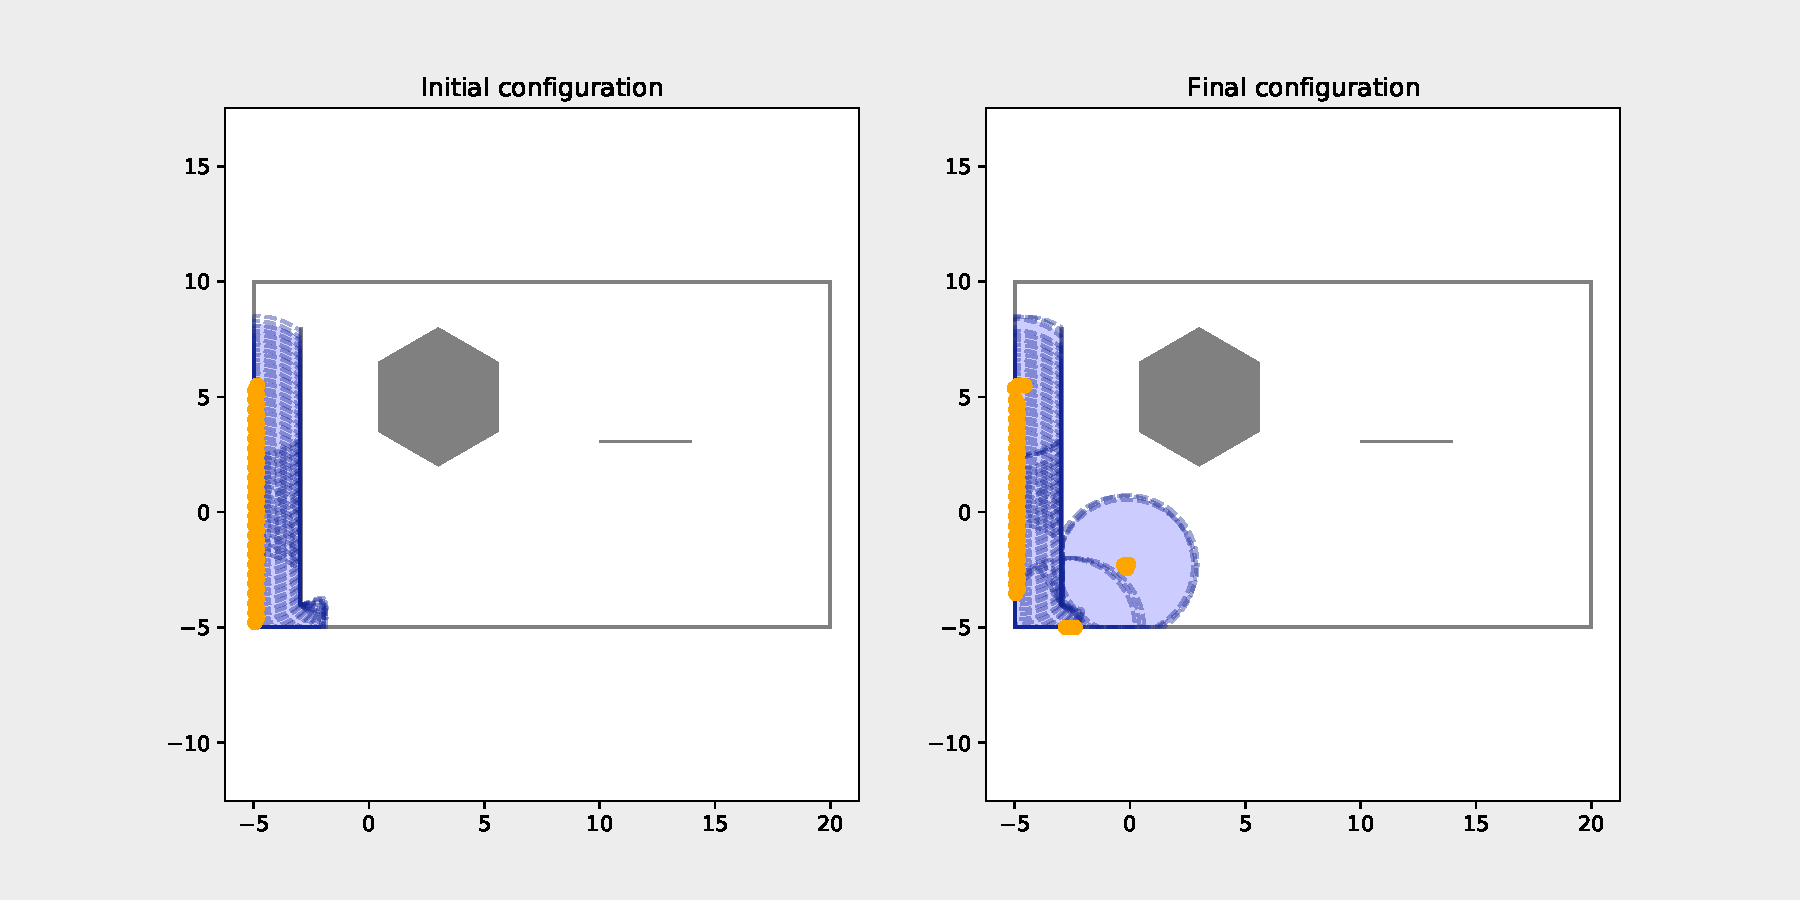
\includegraphics[width=\textwidth]{figs/complexworld_50_agnt_k_1_0_k_2_1_distr.pdf}
  \caption{Initial and final configuration of 50 agents in the Complexworld environment with $k_{1} = k_{2} = 1$ (active dispersion).}
  \label{fig:50_agnt_cw_k_1_0_k_2_1_distr}
\end{figure}

\begin{figure}[H]
  \centering
  \begin{subfigure}[t]{0.5\textwidth}
    \centering
    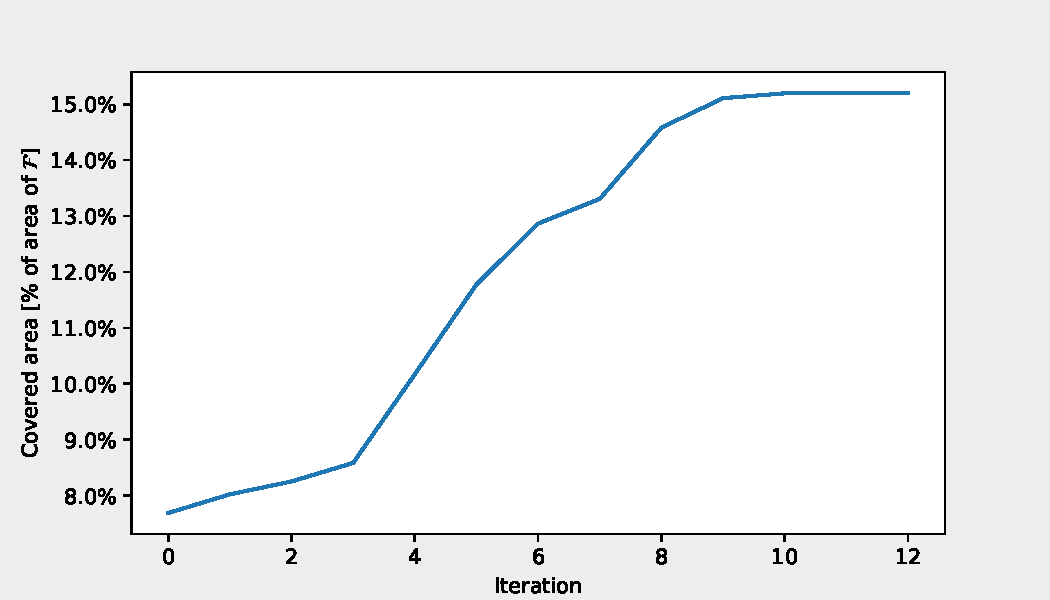
\includegraphics[width=\textwidth]{figs/complexworld_50_agnt_k_1_0_k_2_1_area_traj.pdf}
    \caption{Coverage evolution for 50 agents in the Complexworld environment with $k_{1} = k_{2} = 1$ (active dispersion).}
    \label{fig:50_agnt_cw_k_1_0_k_2_1_a_traj}
  \end{subfigure}%
  ~ 
  \begin{subfigure}[t]{0.5\textwidth}
    \centering
    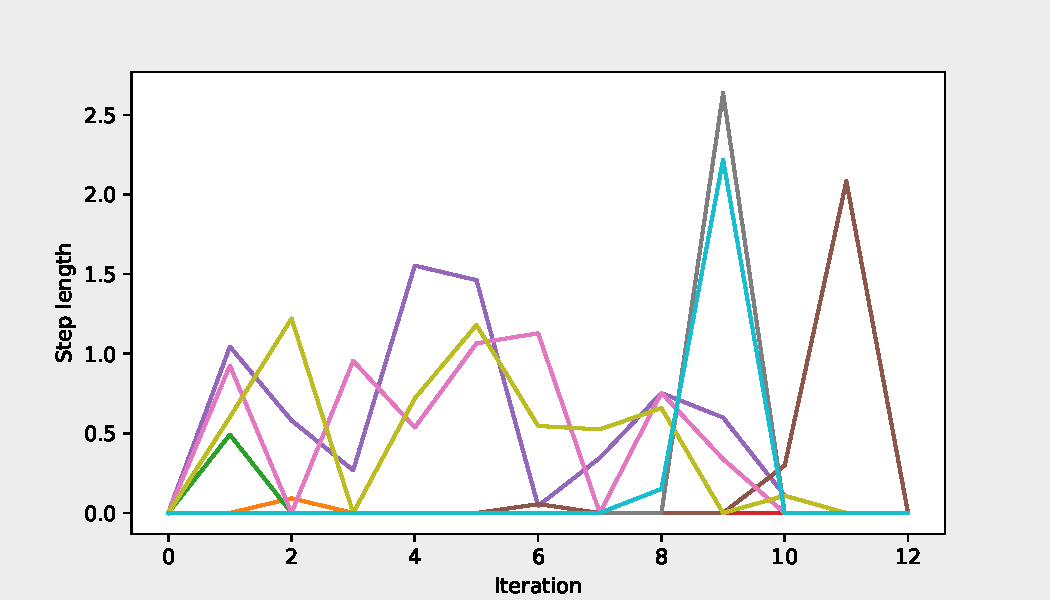
\includegraphics[width=\textwidth]{figs/complexworld_50_agnt_k_1_0_k_2_1_step_traj.pdf}
    \caption{Step length evolution for 50 agents in the Complexworld environment with $k_{1} = k_{2} = 1$ (active dispersion).}
    \label{fig:50_agnt_cw_k_1_0_k_2_1_s_traj}
  \end{subfigure}
  \caption{Coverage percentage and step length evolution for 50 agents in the Complexworld environment when active dispersion is used.}
  \label{fig:50_agnt_cw_evolution}
\end{figure}


\begin{figure}[H]
  \centering
  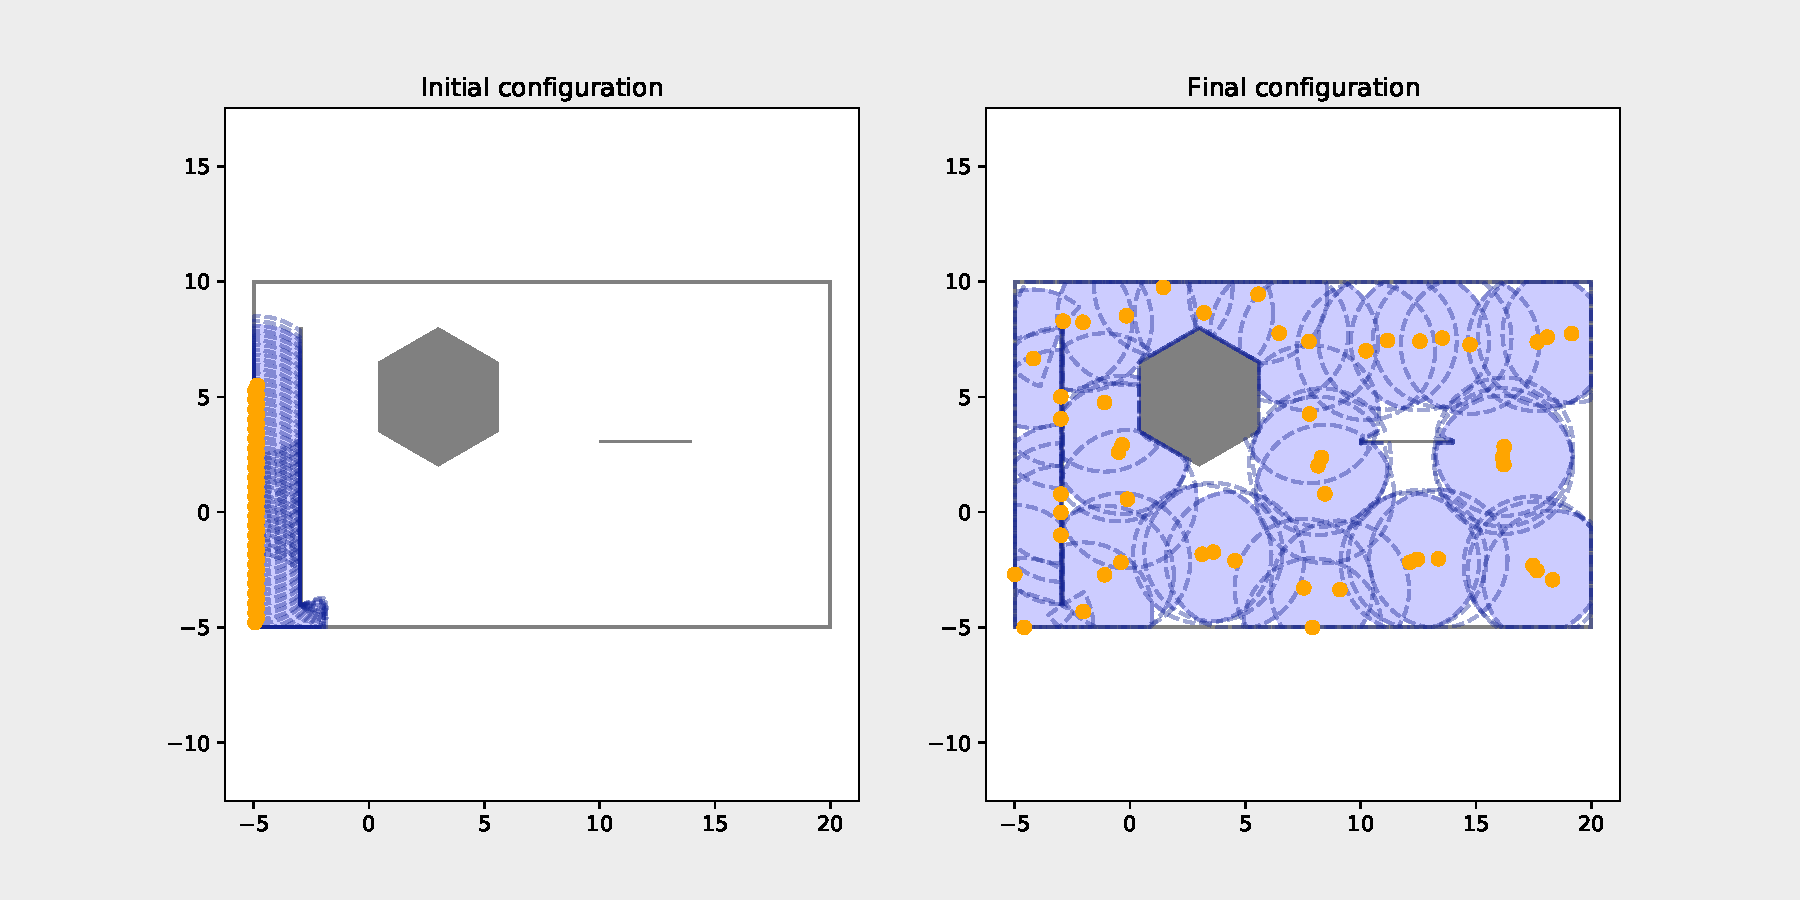
\includegraphics[width=\textwidth]{figs/complexworld_50_agnt_k_1_1_k_2_1_distr.pdf}
  \caption{Initial and final configuration of 50 agents in the Complexworld environment with $k_{1} = k_{2} = 1$ (active dispersion).}
  \label{fig:50_agnt_cw_k_1_1_k_2_1_distr}
\end{figure}

\begin{figure}[H]
  \centering
  \begin{subfigure}[t]{0.5\textwidth}
    \centering
    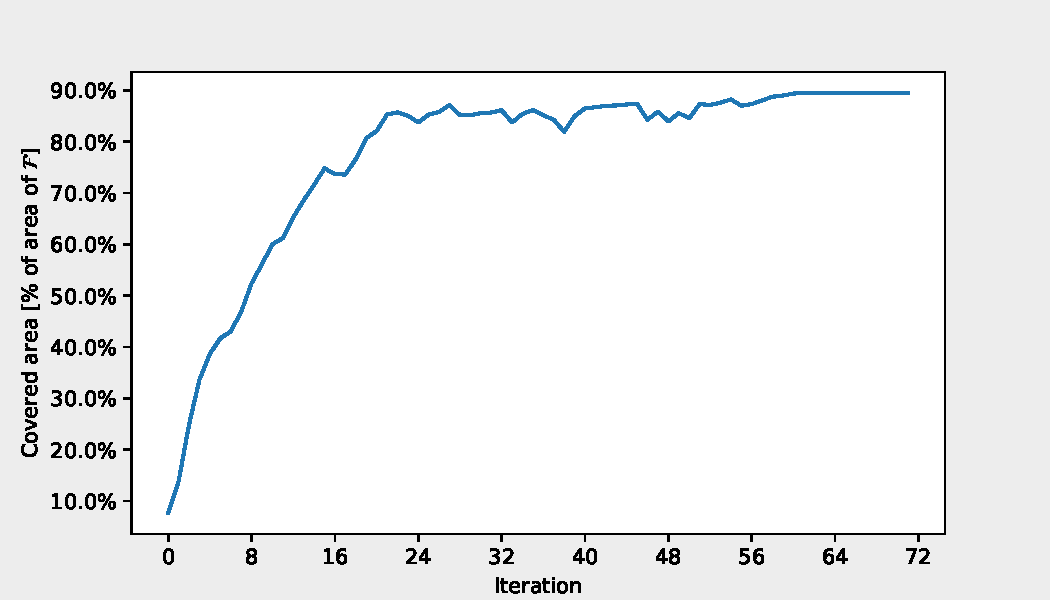
\includegraphics[width=\textwidth]{figs/complexworld_50_agnt_k_1_1_k_2_1_area_traj.pdf}
    \caption{Coverage evolution for 50 agents in the Complexworld environment with $k_{1} = k_{2} = 1$ (active dispersion).}
    \label{fig:50_agnt_cw_k_1_k_2_1_a_traj}
  \end{subfigure}%
  ~ 
  \begin{subfigure}[t]{0.5\textwidth}
    \centering
    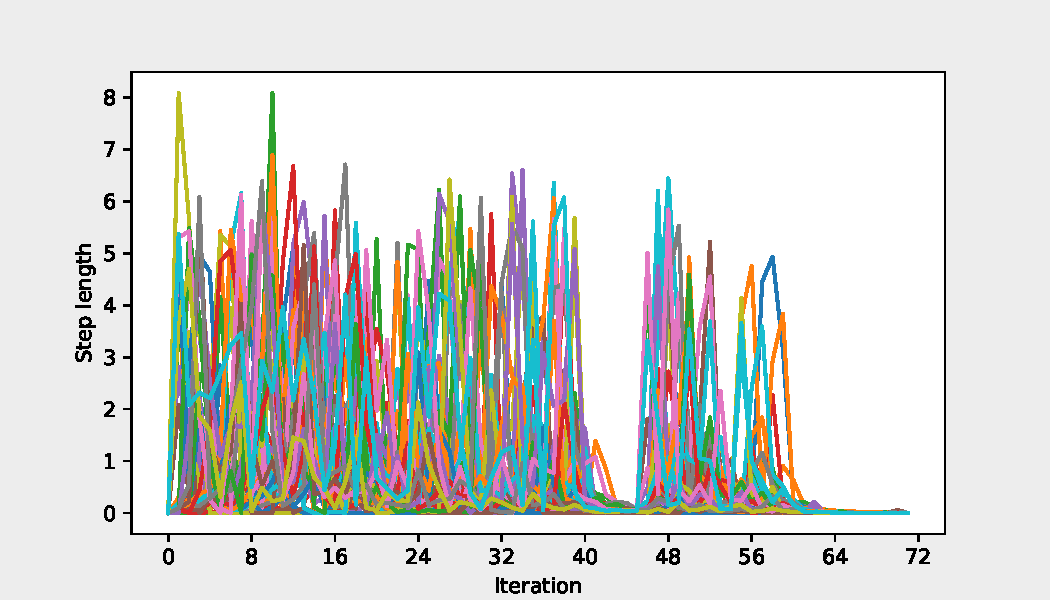
\includegraphics[width=\textwidth]{figs/complexworld_50_agnt_k_1_1_k_2_1_step_traj.pdf}
    \caption{Step length evolution for 50 agents in the Complexworld environment with $k_{1} = k_{2} = 1$ (active dispersion).}
    \label{fig:50_agnt_cw_k_1_1_k_2_1_s_traj}
  \end{subfigure}
  \caption{Coverage percentage and step length evolution for 50 agents in the Complexworld environment when active dispersion is used.}
  \label{fig:50_agnt_tw_evolution_active}
\end{figure}
